\chapter{Cross Section Measurement}

The cross section measurement procedure and results are explained in this section.
After applying selection criteria and kinematic reconstruction, one can count the events to determine
the rate of the $t\bar{t}$ production process.

The cross sections were measured double differentially in bins of the kinematic variables of top-quark and $t\bar{t}$ system.
The first section gives an overview of the background processes for the $t\bar{t}$ production.
The two dimensional unfolding was applied to correct for the detector effect and fluctuations, which is described
in the second section of this chapter.
The double differential cross sections and their definitions are shown in the last section of the chapter.
% \section{Selection of Binning}\label{sec:binning}

\section{Background Subtraction}
This study is performed as counting the events which fulfill certain criteria (e.g. given in chapter \ref{chapt:event_selection} and 
chapter \ref{chapt:kinReco}). Not all of these events are the \textbf{signal events} originating from the $t\bar{t}$ system decay in dileptonic
channel. The final state, which can be misidentified as $t\bar{t}$, may arise from a different process, called \textit{background}
for the specific measurement. In this analysis the background rates are estimated from the simulation and Subtracted 
from the measured event yields:

\begin{equation}\label{eq:bgsub}
 N^{signal\;measured}_{reco} = N^{selected}_{reco} - N^{BG}
\end{equation}

Here the $N^{BG}$ corresponds to the number of background events. It consists of several processes like:

\begin{itemize}
 \item single top production;
 \item Drell-Yan process;
 \item diboson production;
 \item $Z/\gamma^{*} \rightarrow \tau\tau$ production;
 \item $Z/\gamma^{*} \rightarrow ee/\mu\mu$ production;
 \item associated $t\bar{t}\;+\; W/Z/\gamma$ production;
 \item associated $W\;+\;jets$ production;
 \item QCD multijet processes.
\end{itemize}

Whereas all the background yields are only simulated, the estimated rate of the background caused by the Drell-Yan production is 
partially data driven \cite{Chatrchyan:2011nb}. The normalization factor for the simulated Drell-Yan events is determined 
from the comparison of the reconstructed and simulated $Z$-peak. 

After subtracting all the other backgrounds, the number of signal events is multiplied by the factor to cancel the contribution
from the other decay channels of $t\bar{t}$:

\begin{equation}\label{eq:bgsub}
 N^{signal}_{reco} = N^{signal\;measured}_{reco} \cdot \frac{N^{t\bar{t} \rightarrow e\mu}_{reco}}{N^{t\bar{t} \rightarrow e\mu}_{reco} + N^{t\bar{t} \rightarrow other}_{reco}}.
\end{equation}

The whole factor $\frac{N^{t\bar{t} \rightarrow e\mu}_{reco}}{N^{t\bar{t} \rightarrow e\mu}_{reco} + N^{t\bar{t} \rightarrow other}_{reco}}$ was derived
from the simulated data.

%%%%%%%%%%%%%%%%%%%%%%%%%%%%%%%%%%%%%%%%%%%%
%%%%%%%%%%%%%%%%%%%%%%%%%%%%%%%%%%%%%%%%%%%%
%%%%%%%%%%%%%%%%%%%%%%%%%%%%%%%%%%%%%%%%%%%%
\section{Unfolding of the Experimental Results}\label{sec:unfold}

The events after the background  subtraction \ref{eq:bgsub} are grouped to the bins in different variables. However, a finite precision
due to inevitable detector effects and imperfect reconstruction algorithms may lead to incorrect measurement of kinematic properties of the event.
Thus, some fraction of events may be reconstructed in the wrong bins. To present the results independent of the detector effects,
one needs to correct them back.

The whole problem can be described as

\begin{equation}\label{eq:UnfoldProb}
 \tilde{y}_i = \sum_{j = 1}^{m} A_{ij}\tilde{x}_{j} + b_{i}, \;\;\; 1 \leq i \leq n.
\end{equation}

Here the $\tilde{x}_j$ in $m$ bins is a true distribution, independent of the detector effects, which is the aim of the measurement;
$\tilde{y}_i$ in $n$ bins is a distribution which one gets out of the detector and $A_{ij}$ is a matrix of probabilities describing 
the migrations to different bins on the detector level; $b_{i}$ is the background in the bin $i$. 
However, the observed event counts $y_{i}$ may be different from $\tilde{y}_{i}$ due to the statistical fluctuations.
The schematic view of the problem is given in the Figure \ref{fig:scUnf}.

\begin{figure}[t]
  \centering
  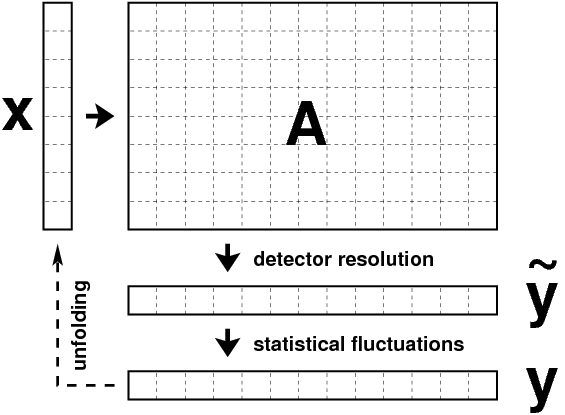
\includegraphics[width=0.4\textwidth]{06_DiffXsec/plots/d12-129f1.png}
  \caption{Schematic view of the problem of migration effects due to the finite precision of the detector and statistical 
  fluctuations. Plot taken from \cite{Schmitt:2012kp}.}
  \label{fig:scUnf}
\end{figure}

The process of restoring the true distribution $\tilde{x}_{j}$ from the known distribution $y_{i}$ which was influenced
by the detector effects and statistical fluctuations is called \textit{unfolding}. To minify these fluctuations the 
\textit{regularisation} procedure is applied. The TUnfold \cite{Schmitt:2012kp} algorithm was used for the
unfolding in this analysis.

\subsection{TUnfold Minimization}\label{ssec:TUmini}

The TUnfold algorithm is using the least square minimization method and the Tikhonov regularization \cite{Tikhonov:1963}. One of the crucial 
constrains for a better performance of the method is that the number of degrees of freedom for the minimization ($n - m$) has to be positive,
or $n > m$. This means that the true unfolded distribution $\tilde{x}_j$ will have coarser binning than the measured one, $y_{i}$.

The unfolding algorithm of the TUnfold determines the stationary point or minimum of the Lagrangian:

\begin{align}
 \mathcal{L}(x, \lambda) & = \mathcal{L}_{1} + \mathcal{L}_{2} + \mathcal{L}_{3}, \;\;\;\;\;\;\;\;\;\; \textrm{where}\\
 \mathcal{L}_{1} & = (\mathbf{y} - \mathbf{A}\mathbf{x})^{T} \mathbf{V_{yy}}^{-1}(\mathbf{y} - \mathbf{A}\mathbf{x}),\\
 \mathcal{L}_{2} & = \tau^{2}(\mathbf{x} - f_{b}\mathbf{x_{0}})^{T} (\mathbf{L^{T}L}) (\mathbf{x} - f_{b}\mathbf{x_{0}}), \\
 \mathcal{L}_{3} & = \lambda(Y -\mathbf{e}^{T}\mathbf{x}) \;\;\;\;\;\;\;\;\;\;\;\;\;\;\;\; \textrm{with} \\
 Y & = \sum_{i} y_{i}, \\
 e_{j} & = \sum_{i} A_{ij}.
\end{align}

The bold symbols here correspond to the matrices and vectors.

The term $\mathcal{L}_{1}$ is expected for the minimization. Vectors $\mathbf{y}$, $\mathbf{x}$ and a matrix $\mathbf{A}$ were
described in the previous section. Representing the migrations from and into different bins of $\mathbf{y}$, the matrix $\mathbf{A}$
is defined from the Monte Carlo\footnote{A matrix $\mathbf{\tilde{A}}$ is
determined from Monte Carlo using the information from the generator particle level and on the reconstructed signal. It describes how many 
migrations there were out and into a certain bin. An extra "zero`` row is added
to the matrix $\mathbf{\tilde{A}}$ containing the information about the count of Monte Carlo events which were generated in some bin of $\mathbf{x}$,
but were not reconstructed in any of the $\mathbf{y}$ bins. \\ The matrix $\mathbf{A}$, which enters the unfolding, is the normalized $\mathbf{\tilde{A}}$
defined as $\mathbf{A}_{ij} = \frac{\tilde{A}_{ij}}{\sum_{j=0}\tilde{A}_{ij}}$ (the normalization includes the "zero'' row).}. An example of such matrix 
is presented in Fig. \ref{fig:migMat}. The $\mathbf{V_{yy}}$ is a covariance matrix of $\mathbf{y}$. 

\begin{figure}[p]
  \centering
  \includegraphics[width=1.0\textwidth]{/home/dolinska/Dropbox/desy_plots/Thesis/Jenya/Plots/Nominal/emu/top_arapidity-top_pt/probabilityMatrix_top_arapidity_vs_top_pt.pdf}
  \caption{Migration matrix for the bins of $p_{T}(t)$ and $|y(t)|$. The binning is the following:
  X axis: the sequences of three bins (1-3, 4-6, 7-9, 10-12, 13-15) correspond to the $p_{T}(t)$ bins $[0\:\:65\:\:130\:\:200\:\:300\:\:500]$ GeV.
          There are 3 $|y(t)|$ bins -- $[0\:\:0.6\:\:1.2\:\:2.5]$ -- in each $p_{T}(t)$ bin.
  Y axis: the sequences of eight bins correspond to the $p_{T}(t)$ bins $[0\:\:20\:\:35\:\:50\:\:65\:\:80\:\:100\:\:130\:\:145\:\:170\:\:200\:\:240\:\:300\:\:350\:\:500]$ GeV.
          There are 8 $|y(t)|$ bins -- $[0\:\:0.2\:\:0.4\:\:0.6\:\:0.8\:\:1.0\:\:1.2\:\:1.5\:\:2.5]$ -- in each $p_{T}(t)$ bin.
  The matrix is obtained from the \MG + \PYTHIA 6 signal sample.}
  \label{fig:migMat}
\end{figure}

The term $\mathcal{L}_{2}$ is responsible for the regularization. It is reducing the effect of the statistical fluctuations of $\mathbf{y}$
during the search of the stationary point of the Lagrangian $\mathcal{L}$. The $\tau^{2}$ is the regularization strength. Matrix $\mathbf{L}$
represents regularization conditions, having $n$ columns and $n_{R}$ rows which corresponds to $n_{R}$ conditions. $f_{b}$ is a normalization 
factor. In a very simple case $f_{b} = 0$, $\mathbf{L}$ is a unity matrix and $\mathcal{L}_{2} = \tau^{2} \parallel x \parallel^{2}$, which
suppresses the large deviations of $\mathbf{x}$ from zero. In case $f_{b} = 1$, the deviations of $\mathbf{x}$ from $\mathbf{x_{0}}$ are
suppressed. For this analysis $f_{b} = 1$ is used and $x_{0}$ corresponds to the generated distribution. It is very important to choose 
the optimal regularization strength, as a very weak strength would not damp the fluctuation effects from $\mathbf{y}$, whereas a very strong 
one will bias $\mathbf{x}$ towards $f_{b}\mathbf{x}_{0}$. The L-curve method \cite{Hansen00thel-curve} and the minimization
of correlation coefficients \cite{VBlobelT} are implemented in TUnfold for an optimal regularization strength choice. 

The idea of the L-curve method is to look at the graph $L_{x}^{curve}$ vs $L_{y}^{curve}$ and choose the $\tau$ from the point with
maximal curvature. The $L_{x}^{curve}$ and $L_{y}^{curve}$ are expressed as follows:

\begin{equation}
 L_{x}^{curve} = log \mathcal{L}_{1},
\end{equation}

\begin{equation}
 L_{y}^{curve} = log \frac{\mathcal{L}_{2}}{\tau^{2}}.
\end{equation}

The method of minimizing the global correlation coefficient chooses the $\tau$ at the point where the average correlation coefficient 
$\sum_{i} \frac{\rho_{i}}{n}$. Here $i$ is the component of $\mathbf{x}$ with length $n$ and $\rho_{i}$ is given as follows:\

\begin{equation}
 \rho_{i} = \sqrt{1 - \frac{1}{(\mathbf{V}_{xx}^{-1})_{ii} (\mathbf{V}_{xx})_{ii}}}.
\end{equation}

$\mathbf{V}_{xx}$ is the covariance matrix for $\mathbf{x}$.

In Fig. \ref{fig:reg_s_m} the example of the choices of regularization strength for both methods are shown.

\begin{figure}[p]
\centering
\begin{subfigure}
  \centering
  \includegraphics[width=0.6\textwidth]{/home/dolinska/Dropbox/desy_plots/Thesis/Jenya/Plots/Nominal/emu/top_arapidity-top_pt/Lcurve_top_arapidity_vs_top_pt.pdf}
\end{subfigure}
\begin{subfigure}
  \centering
  \includegraphics[page=2,width=0.6\textwidth]{/home/dolinska/Dropbox/desy_plots/Thesis/Jenya/Plots/Nominal/emu/top_arapidity-top_pt/logTauRho_top_arapidity_vs_top_pt.pdf}
\end{subfigure}
\caption{Illustration of the choice of the optimal regularization strength with the L-curve method (top) and minimization of correlation coefficient
         (bottom). The red dot represents the point in which the regularization strength $\tau$ is extracted.}
\label{fig:reg_s_m}
\end{figure}

The term $\mathcal{L}_{3}$ is an orthogonal area constrain with a Lagrangian parameter $\lambda$. If $\lambda$ is not set to zero,
which means the area constrain is used, the $\mathbf{x}$ is forced to match the total event count $Y$ correcting for the efficiencies $\mathbf{e}$.
This is used to limit the normalization biases if the data $\mathbf{y}$ follow Poisson's statistics \cite{Cowan98}.

The stationary point of the Lagrangian $\mathcal{L}(\mathbf{x}, \lambda)$ is defined by setting the first derivatives to zero. In case no 
area normalization is performed the Lagrangian $\mathcal{L}$ depends only on $\mathbf{x}$ and $\mathcal{L}_{3}$ term is zero.

\subsubsection{Regularization Strength Studies}

The regularization aims to minimize the fluctuations effects. To check the performance of regularization of the TUnfold, the reconstructed signal
MC sample was unfolded. The outcome of this unfolding should be the generated signal distributions. The number of entries in the reconstructed signal
MC distributions were fluctuated randomly in each bin independently within the statistical uncertainties for data in corresponding bin. 
These statistical uncertainties were assumed to be Gaussian. The fluctuations were performed 3000 times. Each of the 3000 fluctuated distributions 
was unfolded and the following quantities were checked:

\begin{itemize}

 \item \textbf{$\tau$ scan}. The regularization strength $\tau$ is determined using L-curve scan and minimization of correlation coefficients for every
 of the 3000 fluctuated distributions. The regularization strength distributions are shown in
 Fig. \ref{fig:tau_scan}. The regularization strength defined in the L-curve method has multiple peaks which shows instability of $\tau$ choice.
 Such phenomenon is not observed in the results of the minimization of correlation coefficients method. The single value of the regularization strength
 is preferred for all the unfolded distributions. Thus, the minimization of correlation coefficients is used for the cross section determination.
 \begin{figure}[p]
 \centering
 \begin{subfigure}
  \centering
  \includegraphics[width=0.6\textwidth]{/home/dolinska/Dropbox/desy_plots/Thesis/Jenya/Plots/preunfold/emu/top_arapidity-top_pt/L-curve/tauDist_Nominal.png}
 \end{subfigure}
 \begin{subfigure}
  \centering
  \includegraphics[width=0.6\textwidth]{/home/dolinska/Dropbox/desy_plots/Thesis/Jenya/Plots/preunfold/emu/top_arapidity-top_pt/tau-scan-rho/tauDist_Nominal.png}
 \end{subfigure}
 \caption{Distribution of the regularization strength $\tau$ found in a toy experiment with the L-curve method (top) and minimization of correlation coefficient
         (bottom). The red dot represents the regularization strength found by corresponding method in the data.}
 \label{fig:tau_scan}
 \end{figure}
 
 \item \textbf{Relative difference between unfolded and generated values.} The mean number of entries in one bin out of 3000 fluctuated and unfolded distributions
 is being compared to the number of entries in the corresponding generated distribution. The quantity which evaluates this comparison is
 $\frac{\mathbf{x} - \mathbf{x}_{0}}{\mathbf{x}_{average}}$. The average is taken over all the 3000 fluctuated results.
 The distributions of this quantifier in different $p_{T}(t)$ and $|y(t)|$ bins obtained using the L-curve method and minimizing the correlation coefficients 
 are shown in the Fig. \ref{fig:DiffovErr}. The overall relative deviations from zero are not
 higher than 3\%, which means there are no big discrepancies in the unfolding outcome.
 \begin{figure}[h]
 \centering
 \includegraphics[width=0.6\textwidth]{/home/dolinska/Dropbox/desy_plots/Thesis/Jenya/Plots/preunfold/emu/top_arapidity-top_pt/relDiff_Nominal.pdf}
 \caption{The distributions for the 3000 fluctuated and unfolded reconstructed MC signal samples. The distributions are
         presented in bins of top $p_{T}(t)$ and $y(t)$. The results obtained with the L-curve method are marked with red and 
         for the correlation coefficient minimization -- with blue.}
 \label{fig:DiffovErr}
\end{figure}
 
 \item \textbf{RMS over mean error distribution}. The statistics in the same bin in each of the 3000 unfolded
 distributions will differ. To quantify if this spread of the values is not disagreeing with the statistical uncertainties, one can look at the 
 RMS (root mean square) of the values in a certain bin divided by the mean error of these values. This value is expected to equal one.
 The distributions of the RMS over mean errors in different $p_{T}(t)$ and $|y(t)|$ bins obtained using the L-curve method and minimizing the 
 correlation coefficients are shown in the Fig. \ref{fig:RMSovMeanErr}. The results obtained with the L-curve method
 constantly overshoot one. This means, the L-curve method underestimates the errors.
 \begin{figure}[h]
  \centering
  \includegraphics[width=0.6\textwidth]{/home/dolinska/Dropbox/desy_plots/Thesis/Jenya/Plots/preunfold/emu/top_arapidity-top_pt/relDiff_Nominal.pdf}
  \caption{RMS over mean error distributions for the 3000 fluctuated and unfolded reconstructed MC signal samples. The distributions are
         presented in bins of top $p_{T}(t)$ and $|y(t)|$. The results obtained with the L-curve method are marked with red and 
         for the correlation coefficient minimization -- with blue.}
  \label{fig:RMSovMeanErr}
 \end{figure}

\end{itemize}

As a consequence of these studies the minimization of the correlation coefficients method for the regularization strength determination was chosen
to be used in this analysis.

%%%%%%%%%%%%%%%%%%%%%%%%%%%%%%%%%%%%%%%%%%%%
%%%%%%%%%%%%%%%%%%%%%%%%%%%%%%%%%%%%%%%%%%%%
%%%%%%%%%%%%%%%%%%%%%%%%%%%%%%%%%%%%%%%%%%%%
\section{The Double Differential $t\bar{t}$ Production Cross Sections}

\subsection{Cross Section Definition}

After all the corrections are performed, the signal events grouped to different bins are used to define the normalized double differential cross sections
of the $t\bar{t}$ production process:

\begin{equation}\label{eq:ddxsecdef}
 \Delta\;y_{j}: \:\:\:\:\:\:(\frac{1}{\sigma} \frac{d\sigma}{dx\:dy})_{j} = \frac{1}{\sigma} \cdot \frac{1}{\Delta x_{i}} \cdot \frac{N^{signal\:\;unfolded}_{ij}}{\epsilon_{ij} \cdot BR \cdot L}
\end{equation}

Here $\sigma$ is a total cross section, $\epsilon_{ij}$ is the analysis efficiency, $BR$ is a branching ratio of the $t\bar{t}$ dilepton decay channel and $L$ is the luminosity
collected by the CMS detector, which corresponds to 19.7 $fb^{-1}$. The $x$ and $y$ are the kinematic variables in which the cross sections 
are measured. $i$ and $j$ are the number of bins of the variables $x$ and $y$ with the widths $\Delta x_{i}$ and $\Delta y_{i}$.
The number of corrected and unfolded signal events in the $ij^{\textrm{th}}$ bin is the $N^{signal\:\;unfolded}_{ij}$.
Taking to account that the migration matrix is already normalized to the efficiency (see the construction of the matrix in sec. \ref{ssec:TUmini}), 
directly the ratio $N^{signal\:\;unfolded}_{ij} / \epsilon_{ij}$ can be extracted from the unfolding.

The total production cross section $\sigma$ is defined as follows:

\begin{equation}
 \sigma = \frac{N^{signal\;\:unfolded}}{\epsilon \cdot BR \cdot L}.
\end{equation}

\subsection{Phase Space Definition}

The analysis efficiency $\epsilon_{ij}$ (from the eq. \ref{eq:ddxsecdef}) definition is based on the Monte Carlo simulation and predictions.
It may be defined in two different ways:

\begin{itemize}
 \item In the \textbf{full phase space}, taking to account the selection and the detector efficiencies:
 \begin{equation}\label{eq:epsanal}
  \epsilon_{ij} = \mathcal{A} \cdot \epsilon_{ij}^{det},
 \end{equation}
 \\
 where $\mathcal{A}$ is the \textit{acceptance} which defines the effect of the kinematic selection and $\epsilon_{ij}^{det}$ is the detector efficiency part.
 The acceptance is measured on the generator level, to exclude the detector effects:
 \\
 \begin{equation}\label{eq:accep}
  \mathcal{A} = \frac{N^{PS\;selection}_{gen}}{N^{total}_{gen}}.
 \end{equation}
 \\
 Here $N^{total}_{gen}$ is the total number of all generated $t\bar{t}$ signal events,
 The $N_{gen}^{PS\;selection}$ is the number of generated $t\bar{t}$ signal events which pass the so-called phase space selection for the generated leptons and 
 $b$-jets. This selection fully corresponds to the one applied on the reconstruction level (see sec. \ref{sec:sel}) and requires:
 \begin{itemize}
  \item[--] Leptons with $p_{T} \geq 20\;$GeV and $|\eta| \leq 2.4$;
  \item[--] $b$-jets with $p_{T} \geq 30\;$GeV and $|\eta| \leq 2.4$.
 \end{itemize}
 The acceptance extrapolates the measurements outside the phase space selection criteria to the full phase space, taking to account the theory knowledge underlying in the MC generators.
 \\
 The jets on the generator level are defined analogously to the reconstructed jets (see sec. \ref{sec:JetAlgo}) applying the anti-$k_{T}$ algorithm with the 
 cone of $\Delta R$ = 0.5 on the all stable particles after the hadronization. The jets containing the $B$-hadrons originating from the $b$ quarks from the
 top decay are the $b$-jets used for the phase space selection.
 \\
 The detector resolution is defined by cancellation of the selection effects in the following ratio:
 \\
 \begin{equation}\label{eq:epsdet}
  \epsilon_{ij}^{det} = \frac{N^{selected}_{reco}}{N^{PS\;selection}_{gen}}.
 \end{equation}
 \\
 Here $N^{selected}_{reco}$ is the number of simulated reconstructed events. Thus, combining the equation \ref{eq:epsanal}, \ref{eq:accep} and \ref{eq:epsdet},
 the analysis efficiency is expressed as following:
 \\
 \begin{equation}
  \epsilon_{ij} = \frac{N^{selected}_{reco}}{N^{total}_{gen}}.
 \end{equation}
 
 \item In the \textbf{visible phase space}. This efficiency doesn't take to account the selection efficiency, it consists only from the detector efficiency:
 \begin{equation}
  \epsilon_{ij} = \epsilon_{ij}^{det} = \frac{N^{selected}_{reco}}{N^{PS\;selection}_{gen}}.
 \end{equation}
 This efficiency definition doesn't rely on the theoretical predictions for the region outside the visible phase space, but the cross section will depend on
 the selection criteria.
\end{itemize}

The cross sections are measured both in visible and full phase spaces, normalized and not normalized to the total cross section $\sigma$. 


\subsection{Double Differential Production Cross Section Measurement}

The production cross sections were measured double differentially in bins of top transverse momentum, rapidity and Bjorken $x$,
$t\bar{t}$ mass, rapidity and transverse momentum and the angles $\phi$ and $\eta$ between $t$ and $\bar{t}$.
The binning was chosen to have enough entries in each bin at the detector level so that the error could be treated as Gaussian.
It was also checked if the purity, stability and efficiency in each bin are not too low (see the explanation below).

%%%
\subsubsection{Cross sections in bins of $y(t)$ versus $p_{T}(t)$}

The production cross section of the $t\bar{t}$ in bins of the rapidity and the transverse momentum of the top quark was
measured in the bins presented in Fig. \ref{fig:CP_2D_y_pt}. This control distribution is also showing the agreement between 
the data and reconstructed MC $t\bar{t}$ signal. The MC slightly underestimates the data for the lower $p_{T}(t)$ bins and 
in the outer $y(t)$ bins for all the transverse momenta values.

\begin{figure}[t]
  \centering
  \includegraphics[width=0.7\textwidth]{06_DiffXsec/plots/Plots/Nominal/emu/top_rapidity-top_pt/CP_AllBins_top_rapidity_vs_top_pt.pdf}
  \caption{Control distribution of the $y$ of the top quark in bins of the $p_{T}$ of the top quark. The $y$ bins are shown on the top 
  of the plot. The experimental data are marked with the black dots and the reconstructed MC signal is marked with the red area. The error
  bars on the data points represent the statistical uncertainty only. The 
  different background contributions are also shown. On the bottom part of the plot the ratio between data and MC statistics in each bin
  is presented.}
  \label{fig:CP_2D_y_pt}
\end{figure}

The quality of the reconstruction in each bin can be characterized by the three quantities -- \textit{efficiency} $\epsilon$, \textit{purity} $p$ and
\textit{stability} $s$. They are defined the following way:

\begin{equation}
 \epsilon_{ij} = \frac{N^{reco} \cup N_{ij}^{gen}}{N_{ij}^{gen\:tot}},
\end{equation}

\begin{equation}
 p_{ij} = \frac{N_{ij}^{gen} \cup N_{ij}^{reco}}{N_{ij}^{reco}},
\end{equation}

\begin{equation}
 s_{ij} = \frac{N_{ij}^{gen} \cup N_{ij}^{reco}}{N_{ij}^{gen} \cup N^{reco}}.
\end{equation}

All of these quantities are determined from the signal MC. Here $ij$ are the bin numbers in the two dimensions of the variables in which
the cross section is measured. The efficiency 
$\epsilon_{ij}$ is defined as the number of events in intersection of all reconstructed events and events generated in the bin $ij$, 
$N^{reco} \cup N_{ij}^{gen}$, divided by the total number of the generated events $N_{ij}^{gen\:tot}$. 
The efficiency contains the effects of the detector acceptance and the reconstruction efficiency.

The purity $p_{ij}$ is the fraction of the number of the events which were generated and reconstructed in the same bin ($N_{ij}^{gen} \cup N_{ij}^{reco}$)
and the total number of the reconstructed events in this bin ($N_{ij}^{reco}$). The purity describes the migrations inside the bin.
The higher the purity is, the less events migrate inside the bin from the other bins. The highest possible purity value is 1.
The migrations of the events to the different bins are caused by the detector resolution and the reconstruction effects.

The stability $s_{ij}$ is the quotient of the number of events generated and reconstructed in the same bin ($N_{ij}^{gen} \cup N_{ij}^{reco}$) over the 
number of the generated events inside this bin ($N_{ij}^{gen} \cup N^{reco}$). The stability is quantifying the migrations out of the bin. The higher 
the stability is the less events migrate outside this bin to the other bins. The highest possible stability value is 1.

The efficiency, purity and stability are shown in the Fig. \ref{fig:EPS_2D_y_pt}. The reconstruction efficiency and stability are better in the
high $p_{T}$. Although the high rapidity bins have low reconstruction efficiency, the purity and stability there is higher.

\begin{figure}[t]
  \centering
  \includegraphics[width=0.7\textwidth]{06_DiffXsec/plots/Plots/Nominal/emu/top_rapidity-top_pt/EPS_AllBins_top_rapidity_vs_top_pt.pdf}
  \caption{The efficiency (green circles), purity (blue triangles) and stability (red triangles) in bins of the $p_{T}$ and $y$ of the top quark.}
  \label{fig:EPS_2D_y_pt}
\end{figure}

The Fig. \ref{fig:XS_2D_y_pt} represents the production cross sections of the $t\bar{t}$ pair in bins of top rapidity and top transverse momentum.
The experimentally measured cross sections are compared to the MadGraph+Pythia, Powheg+Pythia, Powheg+Herwig and MC@NLO+Herwig predictions.
The overall good agreement between theory predictions and experimental results is observed. MadGraph+Pythia describes the higher $p_{T}$ bins
worth.

\begin{figure}[p]
\centering
\begin{subfigure}
  \centering
  \includegraphics[width=0.49\textwidth]{/home/dolinska/Dropbox/desy_plots/Thesis/Jenya/Plots/FinalPlot/emu/top_arapidity-top_pt/xSec_top_pt_IN_top_arapidity_0.pdf}
\end{subfigure}
\begin{subfigure}
  \centering
  \includegraphics[width=0.49\textwidth]{/home/dolinska/Dropbox/desy_plots/Thesis/Jenya/Plots/FinalPlot/emu/top_arapidity-top_pt/xSec_top_pt_IN_top_arapidity_1.pdf}
\end{subfigure}
\begin{subfigure}
  \centering
  \includegraphics[width=0.49\textwidth]{/home/dolinska/Dropbox/desy_plots/Thesis/Jenya/Plots/FinalPlot/emu/top_arapidity-top_pt/xSec_top_pt_IN_top_arapidity_2.pdf}
\end{subfigure}
\caption{Normalized differential cross sections in bins of top rapidity and transverse momentum.}
\label{fig:XS_2D_y_pt}
\end{figure}

Fig. \ref{fig:corr_matr} presents the correlation matrix $\mathbf{V}_{xx}$ with correlation coefficients for the bins in which the 
cross sections \ref{fig:XS_2D_y_pt} were calculated. There is almost no correlation between the neighboring bins, except for the highest $p_{T}(t)$
bins (shown as the last bins in Fig. \ref{fig:corr_matr}). There is a strong correlation in rapidity observed, which is explained by the strong 
anticorrelation in the last transverse momentum bins.

\begin{figure}[p]
  \centering
  \includegraphics[width=1.0\textwidth]{/home/dolinska/Dropbox/desy_plots/Thesis/Jenya/Plots/Nominal/emu/top_arapidity-top_pt/rhoIJtotal_top_arapidity_vs_top_pt.pdf}
  \caption{Covariance matrix $\mathbf{V}_{xx}$ for the bins of $p_{T}(t)$ and $|y(t)|$. The binning is the following:
  the sequences of three bins (1-3, 4-6, 7-9, 10-12, 13-15) correspond to the $p_{T}(t)$ bins $[0\:\:65\:\:130\:\:200\:\:300\:\:500]$ GeV.
          There are 3 $|y(t)|$ bins -- $[0\:\:0.6\:\:1.2\:\:2.5]$ -- in each $p_{T}(t)$ bin.}
  \label{fig:corr_matr}
\end{figure}

%%%
\subsubsection{Cross sections in bins of $p_{T}(t)$ versus $M(t\bar{t})$}

The other pair of variables in which the $t\bar{t}$ production cross section was measured double differentially is $p_{T}(t)$ and $M(t\bar{t})$.
The control plot, which shows the binning and the comparison between data and simulation, is presented in Fig. \ref{fig:CP_2D_Mtt_pt}. The MC underestimates 
the data for the firs three $p_{T}(t)$ bins and this disagreement grows with the $M(t\bar{t})$. For the last two $p_{T}(t)$ bins, there is
no disagreement observed.

\begin{figure}[t]
  \centering
  \includegraphics[width=0.7\textwidth]{/home/dolinska/Dropbox/desy_plots/Thesis/Jenya/Plots/Nominal/emu/ttbar_mass-top_pt/CP_AllBins_ttbar_mass_vs_top_pt.pdf}
  \caption{Control distribution of the $M(t\bar{t})$ in bins of the $p_{T}$ of the top quark. The $M(t\bar{t})$ bins are shown on the top 
  of the plot. The experimental data are marked with the black dots and the reconstructed MC signal is marked with the red area. The error
  bars on the data points represent the statistical uncertainty only. The 
  different background contributions are also shown. On the bottom part of the plot the ratio between data and MC statistics in each bin
  is presented.}
  \label{fig:CP_2D_Mtt_pt}
\end{figure}

% The efficiency-purity-stability plot is presented in Fig. \ref{fig:EPS_2D_Mtt_pt}.
% 
% \begin{figure}[t]
%   \centering
%   \includegraphics[width=0.7\textwidth]{/home/dolinska/Dropbox/desy_plots/Thesis/Jenya/Plots/Nominal/emu/ttbar_mass-top_pt/EPS_AllBins_ttbar_mass_vs_top_pt.pdf}
%   \caption{The efficiency (green circles), purity (blue triangles) and stability (red triangles) in bins of the $M(t\bar{t})$ and $p_{T}(t)$.}
%   \label{fig:EPS_2D_Mtt_pt}
% \end{figure}

The double differential production cross sections in bins of $M(t\bar{t})$ and $p_{T}(t)$ are presented in Fig. \ref{fig:XS_2D_Mtt_pt}. In general, all the predictions
agree with the data. However, a slight underestimation is observed in the lowest $p_{T}(t)$ bin.

\begin{figure}[p]
\centering
\begin{subfigure}
  \centering
  \includegraphics[width=0.49\textwidth]{/home/dolinska/Dropbox/desy_plots/Thesis/Jenya/Plots/FinalPlot/emu/ttbar_mass-top_pt/xSec_top_pt_IN_ttbar_mass_0.pdf}
\end{subfigure}
\begin{subfigure}
  \centering
  \includegraphics[width=0.49\textwidth]{/home/dolinska/Dropbox/desy_plots/Thesis/Jenya/Plots/FinalPlot/emu/ttbar_mass-top_pt/xSec_top_pt_IN_ttbar_mass_1.pdf}
\end{subfigure}
\begin{subfigure}
  \centering
  \includegraphics[width=0.49\textwidth]{/home/dolinska/Dropbox/desy_plots/Thesis/Jenya/Plots/FinalPlot/emu/ttbar_mass-top_pt/xSec_top_pt_IN_ttbar_mass_2.pdf}
\end{subfigure}
\caption{Normalized differential cross sections in bins of $M(t\bar{t})$ and $p_{T}(t)$. The inner error bands are the statistical uncertainties from the data.
         The outer error bars are the combines statistical and systematical uncertainties on the data.}
\label{fig:XS_2D_Mtt_pt}
\end{figure}

The Fig. \ref{fig:corr_matr_Mtt_pt} shows the correlation matrix $\mathbf{V}_{xx}$ in bins for which the cross sections are calculated. There are no strong correlations
observed.

\begin{figure}[p]
  \centering
  \includegraphics[width=1.0\textwidth]{/home/dolinska/Dropbox/desy_plots/Thesis/Jenya/Plots/Nominal/emu/ttbar_mass-top_pt/rhoIJtotal_ttbar_mass_vs_top_pt.pdf}
  \caption{Covariance matrix $\mathbf{V}_{xx}$ for the bins of $M(t\bar{t})$ and $p_{T}(t)$. The binning is the following:
  the sequences of three bins (1-3, 4-6, 7-9, 10-12, 13-15) correspond to the $p_{T}(t)$ bins $[0\:\:65\:\:130\:\:200\:\:300\:\:500]$ GeV.
          There are 3 $M(t\bar{t})$ bins -- $[340\:\:450\:\:600\:\:1000]$ GeV -- in each $p_{T}(t)$ bin.}
  \label{fig:corr_matr_Mtt_pt}
\end{figure}


%%%
\subsubsection{Cross section in bins of $\Delta\phi(t\bar{t})$ versus $M(t\bar{t})$}

The measurement of the cross section has been performed in bins of the polar angle between top and antitop, $\Delta\phi(t\bar{t})$, and the mass
of the $t\bar{t}$ system, $M(t\bar{t})$.

The control distribution in bins of these variable pair is presented in Fig. \ref{fig:CP_2D_phi_Mtt}. The simulation describes the data well, however
the best agreement is observed in the highest $M(t\bar{t})$ bin.

\begin{figure}[t]
  \centering
  \includegraphics[width=0.7\textwidth]{/home/dolinska/Dropbox/desy_plots/Thesis/Jenya/Plots/Nominal/emu/ttbar_mass-ttbar_delta_phi/CP_AllBins_ttbar_mass_vs_ttbar_delta_phi.pdf}
  \caption{Control distribution of the $M(t\bar{t})$ in bins of the $\Delta\phi$ between the $t$ and $\bar{t}$. The $M(t\bar{t})$ bins are shown on the top 
  of the plot. The experimental data are marked with the black dots and the reconstructed MC signal is marked with the red area. The error
  bars on the data points represent the statistical uncertainty only. The 
  different background contributions are also shown. On the bottom part of the plot the ratio between data and MC statistics in each bin
  is presented.}
  \label{fig:CP_2D_phi_Mtt}
\end{figure}

The Fig. \ref{fig:XS_2D_phi_Mtt} presents the double differential production cross sections of the $t\bar{t}$ pairs in bins of $\Delta\phi(t\bar{t})$ and $M(t\bar{t})$.
All the predictions provide a reasonable description of the measured cross sections. However, the agreement is getting slightly worse for the higher bins of the $M(t\bar{t})$.

\begin{figure}[p]
\centering
\begin{subfigure}
  \centering
  \includegraphics[width=0.49\textwidth]{/home/dolinska/Dropbox/desy_plots/Thesis/Jenya/Plots/FinalPlot/emu/ttbar_mass-ttbar_delta_phi/xSec_ttbar_delta_phi_IN_ttbar_mass_0.pdf}
\end{subfigure}
\begin{subfigure}
  \centering
  \includegraphics[width=0.49\textwidth]{/home/dolinska/Dropbox/desy_plots/Thesis/Jenya/Plots/FinalPlot/emu/ttbar_mass-ttbar_delta_phi/xSec_ttbar_delta_phi_IN_ttbar_mass_1.pdf}
\end{subfigure}
\begin{subfigure}
  \centering
  \includegraphics[width=0.49\textwidth]{/home/dolinska/Dropbox/desy_plots/Thesis/Jenya/Plots/FinalPlot/emu/ttbar_mass-ttbar_delta_phi/xSec_ttbar_delta_phi_IN_ttbar_mass_2.pdf}
\end{subfigure}
\caption{Normalized differential cross sections in bins of $M(t\bar{t})$ and $\Delta\phi(t\bar{t})$. The inner error bands are the statistical uncertainties from the data.
         The outer error bars are the combines statistical and systematical uncertainties on the data.}
\label{fig:XS_2D_phi_Mtt}
\end{figure}

The correlation matrix $\mathbf{V}_{xx}$ in bins used for the cross sections measurement is shown in Fig. \ref{fig:corr_matr_phi_Mtt}. There is no significant correlation
(0.4 at most) observed between any bins.

\begin{figure}[p]
  \centering
  \includegraphics[width=1.0\textwidth]{/home/dolinska/Dropbox/desy_plots/Thesis/Jenya/Plots/Nominal/emu/ttbar_mass-ttbar_delta_phi/rhoIJtotal_ttbar_mass_vs_ttbar_delta_phi.pdf}
  \caption{Covariance matrix $\mathbf{V}_{xx}$ for the bins of $M(t\bar{t})$ and $\Delta\phi(t\bar{t})$. The binning is the following:
  the sequences of three bins (1-3, 4-6, 7-9) correspond to the $\Delta\phi(t\bar{t})$ bins $[0\:\:1.2\:\:2.6\:\:3.14]$ rad.
          There are 3 $M(t\bar{t})$ bins -- $[340\:\:450\:\:600\:\:1000]$ GeV -- in each $\Delta\phi(t\bar{t})$ bin.}
  \label{fig:corr_matr_phi_Mtt}
\end{figure}


%%%
\subsubsection{Cross section in bins of $\Delta\eta(t\bar{t})$ versus $M(t\bar{t})$}

The azimuthal angle between the $t$ and $\bar{t}$ is represented with the pseudorapidity $\Delta\eta(t\bar{t})$. The cross section has been measured
double differentially in bins of $\Delta\eta(t\bar{t})$ and $M(t\bar{t})$.

The control distribution in Fig. \ref{fig:CP_2D_eta_Mtt} shows that the simulation slightly overestimates the experimental data in low $M(t\bar{t})$
and high $\Delta\eta(t\bar{t})$. For the higher $M(t\bar{t})$, however, the situation is completely opposite: the MC underestimates the data and the disagreement
is worse the higher the $\Delta\eta(t\bar{t})$ and $M(t\bar{t})$ are.

\begin{figure}[t]
  \centering
  \includegraphics[width=0.7\textwidth]{/home/dolinska/Dropbox/desy_plots/Thesis/Jenya/Plots/Nominal/emu/ttbar_mass-ttbar_delta_eta/CP_AllBins_ttbar_mass_vs_ttbar_delta_eta.pdf}
  \caption{Control distribution of the $M(t\bar{t})$ in bins of the $\Delta\eta$ between the $t$ and $\bar{t}$. The $M(t\bar{t})$ bins are shown on the top 
  of the plot. The experimental data are marked with the black dots and the reconstructed MC signal is marked with the red area. The error
  bars on the data points represent the statistical uncertainty only. The 
  different background contributions are also shown. On the bottom part of the plot the ratio between data and MC statistics in each bin
  is presented.}
  \label{fig:CP_2D_eta_Mtt}
\end{figure}

The double differential production cross sections in bins of $\Delta\eta(t\bar{t})$ and $M(t\bar{t})$ is presented in Fig. \ref{fig:XS_2D_eta_Mtt}. The \MG + \PYTHIA
prediction shows the worst agreement. There is a slight tendency that the higher the mass is, the more MC underestimates the data for the higher $\Delta\eta(t\bar{t})$.

\begin{figure}[p]
\centering
\begin{subfigure}
  \centering
  \includegraphics[width=0.49\textwidth]{/home/dolinska/Dropbox/desy_plots/Thesis/Jenya/Plots/FinalPlot/emu/ttbar_mass-ttbar_delta_eta/xSec_ttbar_delta_eta_IN_ttbar_mass_0.pdf}
\end{subfigure}
\begin{subfigure}
  \centering
  \includegraphics[width=0.49\textwidth]{/home/dolinska/Dropbox/desy_plots/Thesis/Jenya/Plots/FinalPlot/emu/ttbar_mass-ttbar_delta_eta/xSec_ttbar_delta_eta_IN_ttbar_mass_1.pdf}
\end{subfigure}
\begin{subfigure}
  \centering
  \includegraphics[width=0.49\textwidth]{/home/dolinska/Dropbox/desy_plots/Thesis/Jenya/Plots/FinalPlot/emu/ttbar_mass-ttbar_delta_eta/xSec_ttbar_delta_eta_IN_ttbar_mass_2.pdf}
\end{subfigure}
\caption{Normalized differential cross sections in bins of $M(t\bar{t})$ and $\Delta\eta(t\bar{t})$. The inner error bands are the statistical uncertainties from the data.
         The outer error bars are the combines statistical and systematical uncertainties on the data.}
\label{fig:XS_2D_eta_Mtt}
\end{figure}

The Fig. \ref{fig:corr_matr_eta_Mtt} shows the correlation matrix. 

\begin{figure}[p]
  \centering
  \includegraphics[width=1.0\textwidth]{/home/dolinska/Dropbox/desy_plots/Thesis/Jenya/Plots/Nominal/emu/ttbar_mass-ttbar_delta_eta/rhoIJtotal_ttbar_mass_vs_ttbar_delta_eta.pdf}
  \caption{Covariance matrix $\mathbf{V}_{xx}$ for the bins of $M(t\bar{t})$ and $\Delta\eta(t\bar{t})$. The binning is the following:
  the sequences of three bins (1-3, 4-6, 7-9) correspond to the $\Delta\phi(t\bar{t})$ bins $[0\:\:1.2\:\:2.6\:\:3.14]$ rad.
          There are 3 $M(t\bar{t})$ bins -- $[340\:\:450\:\:600\:\:1000]$ GeV -- in each $\Delta\phi(t\bar{t})$ bin.}
  \label{fig:corr_matr_phi_Mtt}
\end{figure}

%%%
\subsubsection{Cross sections in bins of $p_{T}(t\bar{t})$ versus $|y(t\bar{t})|$}

Another pair of variables in bins of which the cross section was measured is the $p_{T}$ and $|y|$ of the $t\bar{t}$ system. 
The control distribution in bins of the is presented in the Fig. \ref{fig:CP_2D_pttt_ytt}.

% \begin{figure}[t]
%   \centering
%   \includegraphics[width=0.7\textwidth]{/home/dolinska/Dropbox/desy_plots/Thesis/Jenya/Plots/Nominal/emu/ttbar_mass-top_pt/CP_AllBins_ttbar_mass_vs_top_pt.pdf}
%   \caption{Control distribution of the $M(t\bar{t})$ of the top quark in bins of the $p_{T}$ of the top quark. The $M(t\bar{t})$ bins are shown on the top 
%   of the plot. The experimental data are marked with the black dots and the reconstructed MC signal is marked with the red area. The error
%   bars on the data points represent the statistical uncertainty only. The 
%   different background contributions are also shown. On the bottom part of the plot the ratio between data and MC statistics in each bin
%   is presented.}
%   \label{fig:CP_2D_pttt_ytt}
% \end{figure}